
\documentclass[conference]{IEEEtran}
%
\ifCLASSINFOpdf
  \usepackage[pdftex]{graphicx}
  % declare the path(s) where your graphic files are
  % \graphicspath{{../pdf/}{../jpeg/}}
  % and their extensions so you won't have to specify these with
  % every instance of \includegraphics
  % \DeclareGraphicsExtensions{.pdf,.jpeg,.png}
\else
  % or other class option (dvipsone, dvipdf, if not using dvips). graphicx
  % will default to the driver specified in the system graphics.cfg if no
  % driver is specified.
   \usepackage[dvips]{graphicx}
  % declare the path(s) where your graphic files are
  % \graphicspath{{../eps/}}
  % and their extensions so you won't have to specify these with
  % every instance of \includegraphics
  % \DeclareGraphicsExtensions{.eps}
\fi

% *** MATH PACKAGES ***
%
%\usepackage[cmex10]{amsmath}

% *** SPECIALIZED LIST PACKAGES ***
%
%\usepackage{algorithmic}

% *** ALIGNMENT PACKAGES ***
%
%\usepackage{array}

%\usepackage{mdwmath}
%\usepackage{mdwtab}

%\usepackage{eqparbox}


%\usepackage[caption=false]{caption}
%\usepackage[font=footnotesize]{subfig}

% *** FLOAT PACKAGES ***
%
%\usepackage{fixltx2e}

%\usepackage{stfloats}

% *** PDF, URL AND HYPERLINK PACKAGES ***
%
%\usepackage{url}
% correct bad hyphenation here
\hyphenation{op-tical net-works semi-conduc-tor}

\usepackage{url}
\usepackage{hyperref}
\usepackage{caption}
\usepackage{multirow}
\usepackage{array}
\usepackage{lscape}
\usepackage{tikz}
\usepackage{longtable}



\newcommand{\rem}[2]{{\bf [#1] #2}}

\begin{document}
%
% paper title
% can use linebreaks \\ within to get better formatting as desired
\title{A Survey on the Virtual Observatory}


% author names and affiliations
% use a multiple column layout for up to three different
% affiliations
\author{\IEEEauthorblockN{Mauricio
Araya \and Mauricio Solar \and Jonathan Antognini \and Jos\'e Marroqu\'in}}
%\IEEEauthorblockA{Department of Informatics\\
%Universidad Técnica Federico Santa María\\
%Avenida España 1680, Valparaíso, Chile\\
%http://www.inf.utfsm.cl}
%\and
%\IEEEauthorblockN{Diego Mardones}
%\IEEEauthorblockA{Starfleet Academy\\
%San Francisco, California 96678-2391\\
%Telephone: (800) 555--1212\\
%Fax: (888) 555--1212}
%\and
%\IEEEauthorblockN{Karim Pichara}
%\IEEEauthorblockA{Starfleet Academy\\
%San Francisco, California 96678-2391\\
%Telephone: (800) 555--1212\\
%Fax: (888) 555--1212}
%\and
%\IEEEauthorblockN{Ricardo Contreras}
%\IEEEauthorblockA{Starfleet Academy\\
%San Francisco, California 96678-2391\\
%Telephone: (800) 555--1212\\
%Fax: (888) 555--1212}
%\and
%\IEEEauthorblockN{Victor Parada}
%\IEEEauthorblockA{Starfleet Academy\\
%San Francisco, California 96678-2391\\
%Telephone: (800) 555--1212\\
%Fax: (888) 555--1212}}



% conference papers do not typically use \thanks and this command
% is locked out in conference mode. If really needed, such as for
% the acknowledgment of grants, issue a \IEEEoverridecommandlockouts
% after \documentclass

% for over three affiliations, or if they all won't fit within the width
% of the page, use this alternative format:
% 
%\author{\IEEEauthorblockN{Michael Shell\IEEEauthorrefmark{1},
%Homer Simpson\IEEEauthorrefmark{2},
%James Kirk\IEEEauthorrefmark{3}, 
%Montgomery Scott\IEEEauthorrefmark{3} and
%Eldon Tyrell\IEEEauthorrefmark{4}}
%\IEEEauthorblockA{\IEEEauthorrefmark{1}School of Electrical and Computer Engineering\\
%Georgia Institute of Technology,
%Atlanta, Georgia 30332--0250\\ Email: see http://www.michaelshell.org/contact.html}
%\IEEEauthorblockA{\IEEEauthorrefmark{2}Twentieth Century Fox, Springfield, USA\\
%Email: homer@thesimpsons.com}
%\IEEEauthorblockA{\IEEEauthorrefmark{3}Starfleet Academy, San Francisco, California 96678-2391\\
%Telephone: (800) 555--1212, Fax: (888) 555--1212}
%\IEEEauthorblockA{\IEEEauthorrefmark{4}Tyrell Inc., 123 Replicant Street, Los Angeles, California 90210--4321}}




% use for special paper notices
%\IEEEspecialpapernotice{(Invited Paper)}




% make the title area
\maketitle


\begin{abstract}
%\boldmath
This paper presents a short survey on the astronomical Virtual Observatories (VOs) that are 
part of the International Virtual Observatory Alliance (IVOA). From how they are
distributed worldwide to their specialization range on the electromagnetic spectrum, 
we summarize key aspects of the current 19 VO members. 

\end{abstract}
% IEEEtran.cls defaults to using nonbold math in the Abstract.
% This preserves the distinction between vectors and scalars. However,
% if the conference you are submitting to favors bold math in the abstract,
% then you can use LaTeX's standard command \boldmath at the very start
% of the abstract to achieve this. Many IEEE journals/conferences frown on
% math in the abstract anyway.

% no keywords




% For peer review papers, you can put extra information on the cover
% page as needed:
% \ifCLASSOPTIONpeerreview
% \begin{center} \bfseries EDICS Category: 3-BBND \end{center}
% \fi
%
% For peerreview papers, this IEEEtran command inserts a page break and
% creates the second title. It will be ignored for other modes.
\IEEEpeerreviewmaketitle

\section{Introduction}
	The Virtual Observatory (VO) is a international initiative which allows
the access to astronomical files and data centers to astronomers and any person
through Internet. With the standardization of the information and methods is
possible study the astronomical data without the physical requirement of the
tools and location.\\

	In June 2002, was made the International Virtual Observatory Alliance
(IVOA) to ``facilitate the international coordination and collaboration
necessary for the development and deployment of the tools, systems and
organizational structures necessary to enable the international utilization of
astronomical archives as an integrated and interoperating virtual observatory''.
Actually, the IVOA is composed of 19\footnote{On the official website in
\textbf{What is the IVOA} ``the IVOA now comprises 17 VO projects'', but in
\textbf{Member Organizations} appears 19 members listed.} projects of America,
Asia, Europa and Oceania; its members meet two times each year in
Interoperability  Workshops to have discussions face-to-face and resolve
technical questions.\\

	An initiative led by Ph. D. Mauricio Solar alongisde students of
Federico Santa Mar\'{i}a Technical University intends to develop an
astro-informatics platform to manage and analyse intelligently large-scale data
based on the IVOA standards. Due the above, this document aims:

\begin{itemize}
	\item Publicize the distribution of the virtual observatories worldwide.
	\item List the tools developed by the virtual observatories and their
status from the information provided on their official websites on Internet.
	\item Get an idea about what additional tools could be developed to
guarantee fulfilling the main objective\footnote{\textit{``Desarrollo de una
plataforma astro-inform\'{a}tica para la administraci\'{o}n y an\'{a}lisis
inteligente de datos a gran escala''} according to the name of Fondef D11$
\vert $1060 project}.
\end{itemize}

For these purposes were reviewed the official websites of the IVOA and its
members, were read sections of documents about virtual observatories like
``Virtual Observatories, Data Mining, and Astroinformatics'' of Kirk Borne,
George Mason University, among others.\\


%\section{Distribution of IVOA Virtual Observatories Worlwide and its Projects}
\section{IVOA Virtual Observatories Worldwide}


\rem{MA}{Necessity of worldwideness}
\begin{itemize}
\item distributed astronomy facilities
\item unnecessary redundancy of observations and work
\end{itemize}

\rem{MA}{Data Deluge}

\rem{MA}{Why is difficult virtual centers worldwide}
\begin{itemize}
\item to organize the inherent diversity: different goals, working-style, budgets, language
\item why it can be done in science: public data, collaboration, etc
\end{itemize}


\subsection{The IVOA}
\rem{MA}{Check this section}

From June 2002, projects of virtual observatories have come to integrate the
International Virtual Observatory Alliance (IVOA) under the \textbf{Guidelines
for Participation\footnote{The guidelines are available in a paper in PDF and
DOC format from
\url{http://www.ivoa.net/documents/latest/IVOAParticipation.html}}}. These were
founded through national and international governmental and private programs in
collaboration with various centers of scientific studies, universities and
others. Who integrate this project, the Virtual Observatory (VO), share
knowledge between them and the community in a standardized manner. They
themselves are who develop these standards for data exchange and
interoperability. 




The table \ref{table:partners} shows the partners of IVOA to
November 2013.\\

\begin{table}%[h!t]
\centering
%\begin{tabular}{|p{7cm}|p{7cm}|}
\begin{tabular}{|l|l|}
	\hline
	\textbf{Project} & \textbf{URL} \\
	\hline
	NOVA (Argentina) & \url{http://nova.conicet.gov.ar/} \\
	\hline
	ARVO (Armenia) & \url{http://www.aras.am/Arvo/arvo.htm} \\
	\hline
	AstroGrid (United Kingdom) & \url{http://www.astrogrid.org/} \\
	\hline
	Aus-VO (Australia) & \url{http://aus-vo.org.au/} \\
	\hline
	BRAVO (Brazil) & \url{http://www.lna.br/bravo/} \\
	\hline
   CADC (Canada) &
    \url{http://www.cadc-ccda.hia-iha.nrc-cnrc.gc.ca} \\
	\hline
    ChiVO (Chile) & \url{http://www.chivo.cl/} \\
	\hline
    China-VO (China) &
    \url{http://www.china-vo.org/} \\
%	\hline
%    ESA-VO &
%    \url{http://www.sciops.esa.int/} \\
	\hline
	EURO-VO (Europe) & \url{http://www.euro-vo.org/} \\
	\hline
	GAVO (German) & \url{http://www.g-vo.org/} \\
	\hline
	HVO (Hungary) & \url{http://hvo.elte.hu/en/} \\
	\hline
	VObs.it (Italy) & \url{http://vobs.astro.it/} \\
	\hline
	JVO (Japan) & \url{http://jvo.nao.ac.jp/}\\
	\hline
	VO-France (France) & \url{http://www.france-vo.org/} \\
	\hline
	RVO (Russia) & \url{http://www.inasan.rssi.ru/eng/rvo/} \\
	\hline
	SVO (Spain) & \url{http://svo.cab.inta-csic.es/} \\
	\hline
	SA$^3$ (South Africa) & \url{http://www.sa3.ac.za/} \\
	\hline
	UkrVO (Ukrania) & \url{http://www.ukr-vo.org/} \\
	\hline
	VAO (United States) & \url{http://www.usvao.org/} \\
	\hline
	VOI (India) & \url{http://vo.iucaa.ernet.in/~voi/} \\
	\hline
\end{tabular}
\caption{IVOA's partners.}
\label{table:partners}
\end{table}

Almost half of IVOA virtual observatories are supported in Europe\footnote{The
Observatoire Virtuel France is ommited in \textbf{Europe} subsection of
\textbf{List of Virtual Observatories} section by lack of the information.} 9 of
the total; 1 belong to Africa, 1 to Australia, 2 to North America, 3 to South
America and 5 to Asia\footnote{As the mayor part of Rusia's territory is in
Asia, it will be considered like a virtual observatory of Asian continent.}. The
figure 1 shows the distribution of the IVOA's membership per continent.\\

%\begin{figure}%[h]
%\begin{center}
%	\includegraphics[scale=0.6]{img/vo_distribution.png}
%	\caption{International Virtual Observatory Alliance distribution per
%             continent.}
%\end{center}
%\end{figure}

\begin{figure}%[h]
\begin{center}
	\includegraphics[width=0.9\linewidth]{img/VO-worldwide.png}
	\caption{International Virtual Observatory Alliance presence in the world.}
\end{center}
\end{figure}


\rem{JA}{A lot of initiatives converges in one and only VO. Access worldwide to 
scientists.}


\rem{MA}{subsec: Put here the infrastructure and the organizations}
%\subsection{Infrastructure}
%\begin{itemize}
%\item \textbf{EURO-VO}
%\item \textbf{EURO-VO Data Centre Alliance (EuroVO-DCA)}:
%it is supported by the European Union (EU) in the framework of the FP6
%e-Insfraestructure Communication Network Development initiative (project
%RI031675). It began on 1st of September, 2006, and ended on 31th of December,
%2008.
%\item \textbf{EURO-VO Astronomical Infraestructure for Data Access
%              (EuroVO-AIDA)}:
%it is supported by the European Union (UE) in the framework of the FP7
%e-Infrastructure Scientific Research Repositories initiative (project
%RI2121104). It began on 1st of February, 2008, and ended on 31th of July, 2010.
%\end{itemize}

\subsection{Organizations}
\rem{MA}{Funding and Support: important actors of a VO}
\begin{itemize}
	\item \textbf{CVO}
	\item Canadian Astronomy Data Centre
	\item \textbf{VAO}
	\item National Science Foundation, NSF
	\item National Aeronautics and Space Administration, NASA 
	\item Associated Universities, Inc, AUI.
	\item Association of Universities for Reseach in Astronomy, AURA
	\item \textbf{BRAVO}
	\item Brazilian Astronomical Society, SBA
	\item National Institue for Science and Technology in Astrophysics, INCT-A
	\item \textbf{ChiVO}
	\item 5 universities, supported by ALMA, REUNA
	\item \textbf{NOVA}
	\item 8 institutions, National Universitiy of La Plata, Faculty of Astronomical 
		Sciences and Geophysics of la Plata
	\item \textbf{ArVO}
	\item Digital First Byurakan Survey, DFBS
	\item \textbf{AstroGrid}
	\item Particle Physics and Astronomy and Research Council  (PPARC)
	\item Sciency \& Technology Facilities Council (STFC)
	\item \textbf{ESA-VO}
	\item Study
	\item \textbf{EURO-VO}
	\item Continuation of Astrophysical Virtual Observatory, European Commision and six organization
	\item \textbf{GAVO}
	\item Federal Ministry of Education and Research (BMBF)
	\item \textbf{SVO}
	\item Centro de Astrobiología (INTA-CSIC)
	\item Artificial Intelligence Department of the National University of Distance Education
	\item University of Cádiz and Center of Scientific and Academic Services of Catalonia (CESCA)
	\item \textbf{VObs.it}
	\item Italian National Institute for Astrophysics
	\item Information System Units
	\item \textbf{Ukrainian}
	\item Ukrainian Astronomical Association (UAA)
	\item \textbf{SA$^3$}
	\item National Research Fundation
	\item South African Astronomical Observatory
	\item Hartebeesthoek Radio Astronomy Observatory
	\item Square Kilometer Array South Africa 
	\item \textbf{China-VO}
	\item National Astronomical Observatories
	\item Chinese Academy of Sciences
	\item \textbf{JVO}
	\item National Astronomical Observatory of Japan
	\item Fujitsu
	\item \textbf{VOI}
	\item Inter University Center for Astronomy and Astrophysics
	\item Ministry of Communication and Information Technology
	\item \textbf{Aus-VO}
	\item Linkage Infrastructure, Equipment and Facilities
\end{itemize}

\rem{MA}{subsec: Development lines of VOs and data speciality}

% If Chile became part of International Virtual Observatory Alliance, the
% distribution of IVOA's members per continent will be as shown in the figure
% 2. \\

%\begin{comment}
%\begin{figure}%[h]
%\begin{center}
%	\includegraphics[width=110mm]{img/if_chile.png}
%	\caption{International Virtual Observatory Alliance distribution per
%             continent if Chile is accepted.}
%\end{center}
%\end{figure}
%\end{comment}

%Without considering the status of the internal projects of the virtual
%observatories, the membership of Chile would contribute to the cooperation,
%development and interoperability from America in the same percent that Asia.
%Furthermore, this fact would be very significant, because a large numbers of
%astronomical centers like observatories are placed in this country.  For now, is
%intended to work with a certain quantity of data of ALMA.\\


\section{Virtual Observatory by Region}
\label{sec:vo_services}

The IVOA architecture only defines a general framework and
standards that their members should follow, but each VO develop
their own services and tools depending on their specific goals.
The founders and first members are the same countries that have
been developing astronomy and astronomical instruments in the world,
such as in Western Europe, North America, east Asia and Oceania. During the last
few years,
new VOs in other regions were integrated to IVOA, specially in the southern
hemisphere, like the two youngest members: South Africa and Chile.
This offers not only a better worldwide coverage, but the chance of
better exploiting the high-quality data produced by observatories
located in those countries, both locally and globally.

\begin{figure}%[h]
\begin{center}
   \includegraphics[width=0.9\linewidth]{img/VO-worldwide.png}
   \caption{International Virtual Observatory Alliance presence in the world.}
\label{figure:worldview}
\end{center}
\end{figure}

In the rest of this section, the VO initiatives are briefly
described by region (see Figure~\ref{figure:worldview}) to grasp the idea of the advances of
the VO, yet not all of them are included due to space 
constraints.

\subsection{North America}

The \textbf{Canadian Virtual Observatory} (CVO) has largely focus on the CANFAR Virtual Storage
System, which
allows accessing very large resources for both storage and processing, 
using a cloud based framework \cite{Gaudet2011}. 
This is a very generic framework for accessing and processing 
large astronomical data sets that implements most of the
VOSpace standard of IVOA \cite{Graham2007a}. CVO also has implemented
IVOA's data access services like TAP for metadata queries 
and SIA for image access.

A central objective of any VO is to make data accessible by astronomers,
for which the \textbf{US Virtual Astronomical Observatory} (US-VAO) 
offers a web-based service called Data Discovery Tool 
that retrieve data contained in the VO~\cite{McGlynn2013}. 
As a complement, a specific service for discovering time-series data
is also available, called Time Series Search Tool \cite{Graham2012}.
In terms of cloud data processing, the NVO has a Cross-Comparison Tool 
which perform fast positional cross-matches between a large number of 
sources, and a tool for researching multiple sky positions simultaneously (VIM)
\cite{Hanisch2012}.
It also offers a user-side application to find, plot and fit the
Spectral Energies Distributions (SEDs), called Iris~\cite{Laurino2013}.

\subsection{Europe}

One of the most mature VO is \textbf{Astrogrid} (United Kingdom)
\cite{Lawrence2002}, which implements
several IVOA-compliant services and offer very popular user applications
for accessing the VO services~\cite{Lawence2009}.
The implemented services are: \emph{Registry}
for discovering VO services, \emph{Community} to manage user accounts, 
\emph{VOSpace} for virtual file systems and processing, \emph{CEA} for running
generic asynchronous user applications, and \emph{DSA} for metadata/database
access. The very successful stand-alone applications of Astrogrid are 
the VODesktop~\cite{Tedds2008} for data and
TOPCAT \cite{Graham2007} for metadata.
Between other initiatives, Astrogrid offers a middleware platform 
that offers an API for accessing VO services, and a specific 
library for Python scripting.

The \textbf{German Astrophysical Virtual Observatory} (GAVO) is other important VO in Europe that focuses not
only in observational data, but also in theoretical data \cite{Lemson2007}.
The GAVO Data Centre is the service that implements several IVOA standards for 
accessing to the ROSAT archive and other data, for example 
\emph{Registry}, \emph{SIAP}, \emph{SCS}, \emph{VOTable}, \emph{VOPlot}, 
\emph{TAP}, \emph{SSAP}, etc. The services for 
theoretical data includes access to the MultiDark Simulation Database, %\cite{}
% Search
MPA Simulations, %\cite{},
% search
RAVE, % \cite{},
% search
Millenium data, % \cite{},
% search
and TheoSSA, % \cite{}.
% search
Moreover, GAVO offers a full distribution of their server software, called
DaCHS, and maintains SPLAT (a VO-enable spectral analysis tool) and the command line TAP
client \texttt{tapsh}.


The data access services of the \textbf{Observatoires Virtuels France}
(VO-France) are mainly concentrated in the 
CDS Portal, which is a mature service that host popular web-based and
user applications such as Simbad, Aladin, Vizier, Sesame, SimPlay, X-match,
etc., following the IVOA standards. 
Just to highlight a few, Sesame is a name service that query to 
three very complete catalogs and object databases (Simbad, Vizier and Ned),
in order to resolve a name into RA/DEC coordinates. Other interesting 
service is X-match which performs a cross-matching between large amount
of CDS objects or uploaded ones using a grid-based platform.
%search
Another recent VO-France project that is not part of CDS Portal 
is GhoSST, % \cite{},
%search,
which is an experimental database on spectroscopy of solids, that
plans in the near future to be IVOA compliant.

The \textbf{Italian Virtual Observatory} (VObs.it) provides data access to
their archives through the VO-Dance service \cite{Smareglia2001},
which implements several IVOA standards and provides a user-friendly procedure 
to publish astronomical data. An interesting service that VObs.it offers is
VODKA (VO Data Keeping-up Agent), which is a ``new VO actor which monitors the
state of the VO seeking for changes in services and datasets and notifying users
for those changes and updates''. \cite{Laurino2011}

Even though the \textbf{Spanish Virtual Observatory} (SVO) is a younger VO
compared to the previous ones, it
provides access to numerous databases of observational data, and also manages a
theoretical database of synthetic spectra, models and even asteroseismology.
Between the offered IVOA-compliant services we found the VO SED Analyzer (VOSA)
for comparing, managing and processing user or VO photometry-tables,
%search
and the VOSED, which is a SED generator using the VO data.
%search
Also, they provide other interesting services like the Filter Profile Service
database, and the TESELA service \cite{Cardiel2011} to access a catalog 
of blank regions.
The SVO is moving also to data mining projects like the automated classification
of light curves, and the GAIA project that aims to produce a 3D chart of the 
Milky Way. 

The \textbf{Hungarian Virtual Observatory} (HVO) offers a web-based Spectrum
Service \cite{Dobos2006},
that allows access, manipulation and composition of
several measured spectra of astronomical objects. It
also plan to include synthetic spectra generated by
astrophysical models that can be compared with observational
data. Other future plans are automatic photometric redshift 
estimation and performing all these computations in grid clusters. 

The \textbf{Ukrainian Virtual Observatory} (UkrVO)
offers access to the data generated by several Ukranian observatories 
through the Joint Digital Archive (JDA) service. Some of these archives 
(such as DBGPA)
can be accessed through web-based services or through VO applications like
Aladin. The UkrVO offers also user applications like the Variable Stars
Calculator and CoLiTec, which is an automatic detector of asteroids and
comets.
%search

The \textbf{Armenian Virtual Observatory} (ArVO) is strongly based on the
Digital First/Second Byurakan Survey~\cite{Massaro2008}, 
and besides maintaining and making accessible this data to other VOs,
they are focused on generating specialized catalogs like the
blue stellar objects catalog or the late-type star catalog 
\cite{Mickaelian2008}.

\subsection{Asia}

The \textbf{Chinese Virtual Observatory} (China-VO) provides
access to their astronomical archives through the VO-DAS service
that implements IVOA standards like CSC, TAP and Registry. 
Besides this, China-VO offers several services like SkyMouse,
a search engine for astronomical applications, the LAMOST Online
Collaboration Platform and the WWT Community Beijing. It also
offers a wide spectrum of user applications like the FITS Manager\footnote{In
collaboration with VOI} \cite{Cui2012}, 
the FITS Header Archiving System and the VO\_IMPAT
application (an interactive imaging tool). Furthermore, they have developed
some compatibility applications for IVOA standards like the
VOTable Filter for OpenOffice Calc and the 
VOTable to XHTML converter. 

The \textbf{Japanese Virtual Observatory} provides access to theirs
and other VOs resources through the JVO Data Search service 
\cite{Shirasaki2009}, 
including standard IVOA services like SCS, but also more interactive services
such as JVO Sky that allows graphical search, and more low-level
services like JVOQL which allows direct access to the database.
Other offered services are the JVO SExtractor, for detecting sources
from VO files (or external ones), and the JVOSpace service, which is
again a cloud service for storage and processing astronomical files.

The \textbf{Indian Virtual Observatory} (VOI)
concentrates all their web-services in the VOIPortal, which allows
access to several databases within the same framework than other
VOI services such as the Mosaic Service to generate mosaic images 
and PyMorph Service that derive morphological parameters for galaxy
images. VOI has been very prolific in terms of user/web applications, 
such as VOPlot and 
VOMegaPlot for imaging, Astrostat for statistical routines, VOPlatform for
managing astronomical data and VO resources, Android applications, and 
several useful compatibility packages with the IVOA standard as 
the VOTableJava Writer, C++ Parser for VOTable, VOConvert, CSharpFits, etc.
% check http://voi.iucaa.ernet.in/~voi/technical_papers.htm

The \textbf{Russian Virtual Observatory} (RVO) provides access to original
Russian astronomical data and mirrors several astronomical databases 
of other countries. Due the huge diversity of Russian data centers,
RVO mainly concentrates in coordinating the development of services,
tools and new archives of these data centers, with a strong focus in
interoperability and standardization, following the IVOA guidelines
but also developing their own standards and frameworks \cite{Briukhov2005}.
In particular, the Sternberg Astronomical Institute (SAI) is
in charge of the development of VO services, such as the Catalog
Access Services (CAS) that complies with IVOA standards (e.g., ConeSearch,
CrossMatch, SkyNode). Other initiatives of SIA are ADQL2SQL that transform
the Astronomic Data Query Language to PostgreSQL code and the Q3C package
to indexing large astronomical databases in an efficient PostgreSQL 
database.

\subsection{Oceania}
As most VOs, the \textbf{Australian Virtual Observatory} (Aus-VO) offers a 
basic conesearch (SCS) service to access to their archive under the
IVOA standards. Other
services include \emph{SkyCat}, which is an extensible 
astronomical catalogue server, 
and \emph{Volume}, a web application to visualize VOTables in several 
coordinate systems.
%check http://aus-vo.org/paper_trail/papers
Other projects of Aus-VO include a Remote Visualization
System (RVS) for imaging and analysis, a 	
Distributed Volume Renderer (DVR) that renders larger-than-memory volumetric 
datasets on the grid \cite{Beeson2003},
and a cross-matching service based on Machine Learning algorithms.
Currently, the efforts of the Aus-VO are concentrated in a relatively
new project called All-Sky Virtual 
Observatory\footnote{http://www.asvo.org.au/}.

\subsection{Africa}
The \textbf{South African Astroinformatics Alliance} (SA$^3$) 
is a recently added member of IVOA, that aims 
to facilitate access by the astronomical community to
multi-wavelength astronomical data and tools.
Currently, SA$^3$ provides a very complete list of the available datasets and
tools in other VOs, and is expected that it will contribute with their own
applications in the near future.

\subsection{South America}

The \textbf{Brazilian Virtual Observatory} (BRAVO) is working in several
scientific-based project \cite{CarvalhoXXXX} such as a spectral synthesis 
application to
estimate de physical properties of galaxies (STARLiGHT), a tool 
for obtaining interstellar extinction (GALExtin), a photometric redshift
calculator (Zphot), between others. Besides that, BRAVO plans to develop
grid and cloud applications for data mining, based on HPC technology.

The \textbf{Nuevo Observatorio Virtual Argentino} (NOVA) is a young
VO that offers IVOA-compliant registry and data access to surveys and
spectral data. The main technicals goals of NOVA is to develop its portal
within the grid infrastructure, and to produce an efficient interface for
astronomers.

The younger member of IVOA is the \textbf{Chilean Virtual Observatory} (ChiVO),
which plans to become an important data access node to the large amount
of astronomical data generated in Chile. ChiVO is also developing analysis
tools based on Machine Learning and Artificial Intelligence algorithms,
which could naturally be offered as cloud and grid-based services.

\subsection{International Organizations}

The \textbf{European Virtual Observatory} (EURO-VO) offers support and funding
for the European Community VOs.  It works by executing collaboration and
development projects between the VOs with an specific topic, such as ICE
(International Cooperation Empowerment), % \cite{},
%search
AIDA (Astronomical Infrastructure for Data Access),% \cite{},
%search
DCA (Data Centre Alliance), and % \cite{}, and
%search
VOTECH (Virtual Observatory Technology). % \cite{}.
Currently, the EURO-VO is executing the project CoSADIE (Collaborative and
Sustainable Astronomical Data Infrastructure for Europe), which offers 
support, documentation and guidance for astronomers and VO members.
Due its nature, the EURO-VO is a very important member for IVOA, because
it encourages the standardization and collaboration of European VOs.

The \textbf{European Space Agency Virtual Observatory} (ESA-VO) aims to be the
VO end-point for all the space-based astronomy.  It is an active member of the
EURO-VO, providing not only data access and expertise for space-based astronomy,
but generic tools that are useful for all VOs. In fact, the official resource
registry of the EURO-VO is developed and maintained by ESA-VO. 
%search
Between the tools that ESA-VO has developed, there is the \emph{DALToolKit},
that allows to publish in the VO following the DAL protocol, and \emph{VOSpec},
which is a multi-wavelength spectral analysis tool with access to atomic and
molecular databases, spectra and theoretical models registered in the VO.
%search






\section{Platforms for the Astronomical Data}
Most of virtual observatories usually contribute to development of tools for for
national astronomical instruments. These tools can be new source codes for the
exploitation of the capability of some specific instrument, facilitation or
improvement of the queries, reading, writing, conversion of the astronomical
data of files like VOTable, ASCII and FITS formats, among other. As the IVOA 's
member work in Working Groups, belong to another collaboration group and have
non-VO partners, there is a direct or indirect contribution among projects
around the world.\\

Not all virtual observatories projecst have a online or offline platform where
the astronomers, scientists, researches and other can do their queries about
astronomical data. As the the Chilean Virtual Observatory intends to develop an
astro-informatics platform to manage and analyse intelligently the large-scale
data based on the IVOA standards, in first place, the IVOA's projects like it
are cuantified in the table \ref{table:vo_platforms} with the respective query
links and in second place, as the ChiVO will initially work the ALMA's data, are
identified in the same table which of them have access to the same AlMA's
spectrum range\footnote{The spectrum range of ALMA is initially in 400 $ \mu $m
to 3 mm.}.\\

\begin{table}%[h!t]
\centering
\begin{tabular}{|m{2cm}|m{4.5cm}|m{1.5cm}|m{6cm}|}
    \hline
    \textbf{VO} & \textbf{Database's name} & \textbf{Type} & \textbf{URL}
    \\
    \hline
    \multirow{2}{*}{ArVo} & Aladin & Offline & \\
    \cline{2-4}
     & DataScope & Online 
     & \url{http://heasarc.gsfc.nasa.gov/cgi-bin/vo/datascope/init.pl} \\
     \hline
    \multirow{3}{*}{China-VO} & VO Data Access Service (VO-DAS) & Offline & \\
    \cline{2-4}
     & SkyMouse & Online & \url{http://skymouse.china-vo.org/} \\
     \cline{2-4}
     & Chinese Astronomical Data Center & Online 
     & \url{http://casdc.china-vo.org/?locale=en} \\
     \hline
    \multirow{4}{*}{NOVA} & ICATE Multispectral observations Online & Online 
    & \url{http://nova.iafe.uba.ar/icatespec/q_ssa_mixc/web_ms/form} \\
    \cline{2-4}
     & ICATE spectroscopic observations Online & Online
     & \url{http://nova.iafe.uba.ar/icatespec/q_ssa_mixc/web/form} \\
     \cline{2-4}
     & ICAte spectroscopic observations SSAP & Online
     & \url{http://nova.iafe.uba.ar/icatespec/q_ssa_mixc/ssa/form} \\
     \cline{2-4}
     & Very Large Array (VLA) Observations at IAFE & Online 
     & \url{http://nova.iafe.uba.ar/iafevla/q/im/form} \\
     \hline
\end{tabular}
\caption{Online and offline platforms for astronomical data under IVOA
         standards.}
\label{table:vo_platforms}
\end{table}


\section{Virtual Observatory in the Electromagnetic Spectrum}

Most of virtual observatories usually contribute to development of tools for
for national astronomical instruments. These tools can be new source codes for
the exploitation of the capability of some specific instrument, facilitation or
improvement of the queries, reading, writing, conversion of the astronomical
data of files like VOTable, ASCII and FITS formats, among other. 
This means that each VO concentrates in providing services for specific
data types, which in astronomy are highly correlated with the wavelengths values
on which their work. This section surveys the ranges for which 
each virtual observatory is developing their tools, 

\begin{landscape}
\begin{figure}%[h]
\begin{center}
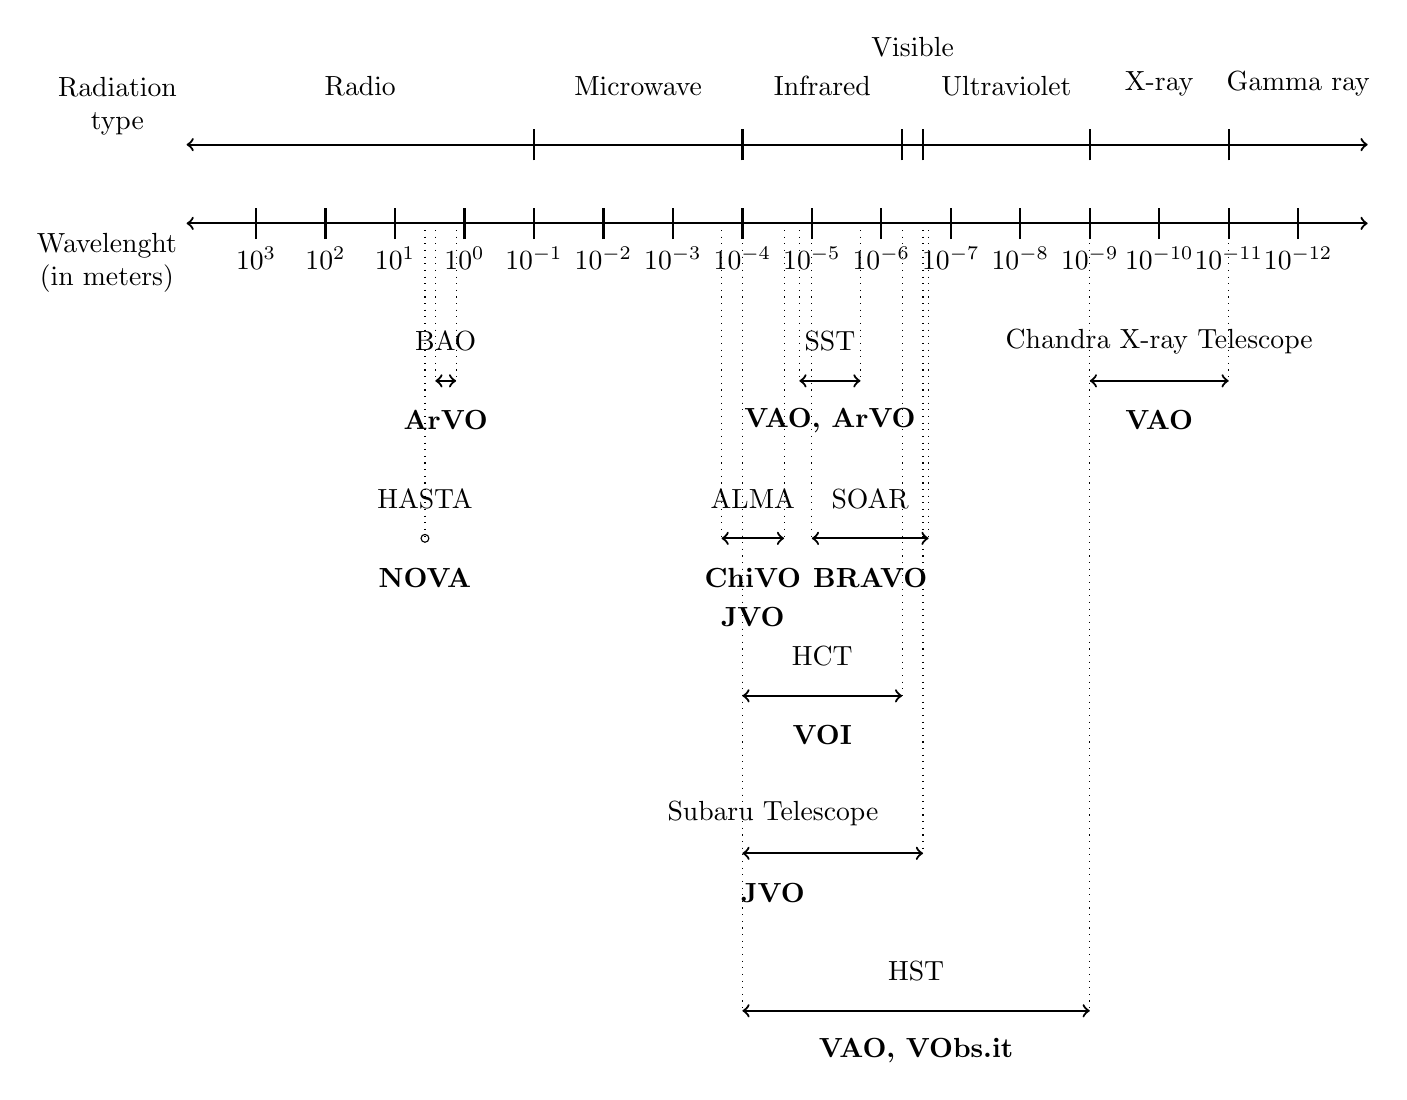
\begin{tikzpicture}
\pgfmathsetmacro{\lineLenght}{15}
\pgfmathsetmacro{\lineDivNum}{17}
\pgfmathsetmacro{\markPlace}{\lineLenght/\lineDivNum}
\def\limitsList{5,8,10.3,10.6,13,15}
\def\regionArray{{2.5,(5+8)/2,(8+10.3)/2,(10.3+10.6)/2,(10.6+13)/2,(13+15)/2,
                  (15+17)/2}}
\foreach \x in {0,1} {
  \draw[<->,thick] (0,\x) -- (\lineLenght,\x);
}
\foreach \x in \limitsList {
  \draw[thick] (\x*\markPlace,0.8) -- (\x*\markPlace,1.2);
}
\foreach \x in {1,2,...,16} {
  \pgfmathtruncatemacro{\b}{\x-2*\x+4} 
  \draw[thick] (\x*\markPlace,-0.2) -- (\x*\markPlace,0.2)
  node[pos=-0.6]{$10^{\b}$};
}
\node [anchor=north east,align=center] at (0,0) {Wavelenght\\(in meters)};
\node [anchor=south east,align=center] at (0,1) {Radiation\\type};
\node [above] at (\regionArray[0]*\markPlace,1.5) {Radio};
\node [above] at (\regionArray[1]*\markPlace,1.5) {Microwave};
\node [above] at (\regionArray[2]*\markPlace,1.5) {Infrared};
\node [above] at (\regionArray[3]*\markPlace,2) {Visible};
\node [above] at (\regionArray[4]*\markPlace,1.5) {Ultraviolet};
\node [above] at (\regionArray[5]*\markPlace,1.5) {X-ray};
\node [above] at (\regionArray[6]*\markPlace,1.5) {Gamma ray};

% Spectrum value or range for each instrument where some virtual observatory
% contributes

\pgfmathsetmacro{\factor}{\markPlace/2}
% ALMA
\draw[<->,thick] (7.7*\markPlace,-4) -- (8.6*\markPlace,-4);
\pgfmathparse{multiply(8.6-7.7,\factor)}
\node at (\pgfmathresult+7.7*\markPlace,-3.5) {ALMA};
\node at (\pgfmathresult+7.7*\markPlace,-4.5) {\textbf{ChiVO}};
\node at (\pgfmathresult+7.7*\markPlace,-5.0) {\textbf{JVO}};
 BAO
\draw[<->,thick] (3.58*\markPlace,-2) -- (3.88*\markPlace,-2);
\pgfmathparse{multiply(3.88-3.58,\factor)}
\node at (\pgfmathresult+3.58*\markPlace,-1.5) {BAO};
\node at (\pgfmathresult+3.58*\markPlace,-2.5) {\textbf{ArVO}};
% Chandra X-ray Telescope 
\draw[<->,thick] (13*\markPlace,-2) -- (15*\markPlace,-2);
\pgfmathparse{multiply(15-13,\factor)}
\node at (\pgfmathresult+13*\markPlace,-1.5) {Chandra X-ray Telescope};
\node at (\pgfmathresult+13*\markPlace,-2.5) {\textbf{VAO}};
% HASTA 
\node at (3.4312*\markPlace,-4) [inner sep=1pt,circle,draw] {};
\node at (3.4312*\markPlace,-3.5) {HASTA};
\node at (3.4312*\markPlace,-4.5) {\textbf{NOVA}};
% HCT
\draw[<->,thick] (8*\markPlace,-6) -- (10.3*\markPlace,-6);
\pgfmathparse{multiply(10.3-8,\factor)}
\node at (\pgfmathresult+8*\markPlace,-5.5) {HCT};
\node at (\pgfmathresult+8*\markPlace,-6.5) {\textbf{VOI}};
% HST  
\draw[<->,thick] (8*\markPlace,-10) -- (13*\markPlace,-10);
\pgfmathparse{multiply(13-8,\factor)}
\node at (\pgfmathresult+8*\markPlace,-9.5) {HST};
\node at (\pgfmathresult+8*\markPlace,-10.5) {\textbf{VAO, VObs.it}};
% SOAR 
\draw[<->,thick] (9*\markPlace,-4) -- (10.68*\markPlace,-4);
\pgfmathparse{multiply(10.68-9,\factor)}
\node at (\pgfmathresult+9*\markPlace,-3.5) {SOAR};
\node at (\pgfmathresult+9*\markPlace,-4.5) {\textbf{BRAVO}};
% SST
\draw[<->,thick] (8.82*\markPlace,-2) -- (9.7*\markPlace,-2);
\pgfmathparse{multiply(9.7-8.82,\factor)}
\node at (\pgfmathresult+8.82*\markPlace,-1.5) {SST};
\node at (\pgfmathresult+8.82*\markPlace,-2.5) {\textbf{VAO, ArVO}};
% Subaru Telescope
\draw[<->,thick] (8*\markPlace,-8) -- (10.6*\markPlace,-8);
\node at (\pgfmathresult+8*\markPlace,-7.5) {Subaru Telescope};
\node at (\pgfmathresult+8*\markPlace,-8.5) {\textbf{JVO}};

% Perpendicular long dotted lines

\def\firstLinesEnds{3.58,3.88,8.82,9.7,13,15}
\foreach \x in \firstLinesEnds {
  \draw[dotted] (\x*\markPlace,0) -- (\x*\markPlace,-2);
}
\def\secondLinesEnds{3.4312,7.7,8.6,9,10.68}
\foreach \x in \secondLinesEnds {
  \draw[dotted] (\x*\markPlace,0) -- (\x*\markPlace,-4);
}
\draw[dotted] (8*\markPlace,0) -- (8*\markPlace,-6);
\draw[dotted] (10.3*\markPlace,0) -- (10.3*\markPlace,-6);
\draw[dotted] (8*\markPlace,0) -- (8*\markPlace,-8);
\draw[dotted] (10.6*\markPlace,0) -- (10.6*\markPlace,-8);
\draw[dotted] (8*\markPlace,0) -- (8*\markPlace,-10);
\draw[dotted] (13*\markPlace,0) -- (13*\markPlace,-10);
\end{tikzpicture}
\caption{Virtual observatories that contributes to specifics astronomical
instruments.}
\end{center}
\label{figure:wavelength}
\end{figure}
\end{landscape}

In Figure \ref{figure:wavelength}, the different types of
radiation (in order) with their common names are shown. Below, the value of
the wavelengths in meters and the respective telescope/instrument are presented. 

%A higher $ \lambda $
%value is related with a lower frequency and a
%lower $ \lambda $ is related with a higher frequency. 
%The electromagnetic
%spectrum value or range for each instrument (above) and virtual observatory
%(below) is represented with a dot or line, respectively.\\

%\scriptsize
%\begin{table*}[h!t]
%\centering
%\begin{tabular}{|p{1cm}|p{4cm}|p{5cm}|p{6cm}|}
%    \hline                                                                      
%    \textbf{VO} & \textbf{Instrument} & \textbf{Location} &
%    \textbf{Spectrum value or range} \\
%    \hline                                                                      
%    BRAVO & Southern Astrophysical Research
%    Telescope (SOAR) & Cerro Pach\'{o}n, Chile & blue (320 nm) to near infrared
%    \cite{website:SOAR_EMS} \\
%    \hline                                                                      
%    NOVA & H-Alpha Solar Telescope for
%    Argentina (HASTA) & Leoncito, San Juan, Argentina & H-Alpha (656.28 nm)
%    \cite{website:HASTA_EMS} \\
%    \hline
%    ChiVO & Atacama Large Milimeter/submilimeter
%    Array (ALMA) & Llano de Chajnantor Observatory, Atacama Desert, Chile &
%    initially in 400 $ \mu $m to 3 mm \cite{website:ALMA_EMS} \\
%    \hline
%    \multirow{3}{3cm}{VAO} & Hubble Space
%    Telescope (HST) & 569 km above the surface of Earth & near-ultraviolet,
%    visible and near-infrared light with WFC3; ultraviolet light with COS;
%    visible light with ACS; ultraviolet, visible and near-infrared light with
%    STIS; infrared light with NICMOS \cite{website:HST_EMS} \\
%     \cline{2-4}
%     & Chandra X-ray Observatory & 139,000 km above the surface of Earth & X-ray
%     \cite{website:Chandra_EMS} \\
%     \cline{2-4}
%     & Spitzer Space Telescope (SST) & 176,602,814 km above the surface of Earth
%     \cite{website:SST_EMS_1} & 3 $ \mu $m to 180 $ \mu $m
%     \cite{website:SST_EMS_2} \\
%    \hline
%    ArVO & Byurakan Astrophysical Observatory
%    (BAO) & Mount Aragats, Armenia & 1.2 m and 4.2 m \cite{website:BAO_EMS} \\
%    \hline
%    ArVO & Spitzer Space Telescope (SST) &
%    176,602,814 km above the surface of Earth & 3 $ \mu $m to 180 $ \mu $m \\
%    \hline
%    Vobs.it & Hubble Space Telescope (HST) & 569
%    km above the surface of Earth & near-ultraviolet, visible and near-infrared
%    light with WFC3; ultraviolet light with COS; visible light with ACS;
%    ultraviolet, visible and near-infrared light with STIS; infrared light with
%    NICMOS \\
%    \hline
%    \multirow{2}{3cm}{UkrVO} & Main Astronomical
%    Observatory (MAO) & Kiev, Ukraine & \\
%     \cline{2-4}
%     & Mykolaiv Astronomical Observatory & Mykolaiv, Ukraine & \\
%    \hline
%    \multirow{3}{3cm}{JVO} & Subaru Telescope &
%    Mauna Kea, Big Island, Hawaii & visible and infrared light
%    \cite{website:Subaru_EMS} \\
%     \cline{2-4}
%     & Sloan Digital Sky Survey (SDSS) & Sacramento Mountains, Sunspot, New
%     Mexico, USA & \\
%     \cline{2-4} 
%     & Atacama Large Milimeter/submilimeter Array (ALMA) & Llano de Chajnantor
%     Observatory, Atacama Desert, Chile & initially in 400 $ \mu $m to 3 mm \\
%    \hline
%    VOI & Himalayan Chandra Telescope (HCT) & Mount
%    Saraswati, Digpa-ratsa Ri, Hanle, India & infrared light 
%    \cite{website:HCT_EMS} \\
%    \hline
% \end{tabular}
%\caption{Virtual observatories that contributes to specifics astronomical
%instruments.}
%\label{table:vo_EMS}
%\end{table*}
%%\end{longtable}
%%\end{center}
%\normalsize



\section{Conclusions and Recommendations}
%At present the distribution of the virtual observatories in the world is not
%related with the astronomical installations, e.g., only ESO (European Souther
%Observatory) operates in three places in the north of Chile: La Silla, Paranal
%and
%Chajnantor\footnote{\url{http://www.eso.org/public/chile/about-eso/cooperation.html}},
%but there still does not exist the presence of the Virtual Observatory (VO).
%The 47\% of virtual observatories have been founded by the members of European
%Community.\\

The membership of IVOA does not
guarantee a constant contribution from its members: the alliance only 
intends to share the astronomical
knowledge between them and the community in a standardized manner. 
In fact, during this research, we have realized that several VOs have not 
updated the status of their projects, and moreover several official sources 
or data is not accessible from a web platform. This paper intent to be
a first step to keep an updated registry of services, tools and projects
developed by the different VOs. 

%The development and implementing of a virtual observatory in Chile is urgent.
%Chile is an astronomer's
%paradise\footnote{\url{http://www.bbc.co.uk/news/world-latin-america-14205720}}.
%A platform under the IVOA's standards from there allows to facilitate the
%Chileans and global astronomical contributions, among others.\\

%Countless of tools could be developed from a Chilean virtual observatory. These
%applications would respond to the currents and future needs for any member of
%IVOA. The International Virtual Observatory Alliance has the Working Groups
%which works to development the standards that would later all members will be
%submitted.\\


\bibliographystyle{plain}
\bibliography{gcv2014}

%\appendix

%\subsection{Summary of Tools and Projects}

The standards and services of a VO are meant to be used in the end 
by applications. The Applications working group have defined only two major
standards for application interoperability beyond the services standards: 
(1) the Simple Application Messaging Protocol (SAMP), and (2) the VOTable
format. These standards, plus all the other protocols and standards 
allows VO-compliant tools to be developed, which are the end-points for
science production. In the next table we summarize the most used tools
and they status.

%%%%%%%%%%%%%%%%%%%%%%%%%%%%%%%%%%%%%%%%%%%%%%%%%%%%%%%%%%%%%%%%%%%%%%%%%%%%%%%%%
%%%%%%%%%%%%%%%%%%%%%%%%%%%%%%%%%$Data Access%%%%%%%%%%%%%%%%%%%%%%%%%%%%%%%%%%%%
%%%%%%%%%%%%%%%%%%%%%%%%%%%%%%%%%%%%%%%%%%%%%%%%%%%%%%%%%%%%%%%%%%%%%%%%%%%%%%%%%
\begin{table*}[h!t]
	\centering
	\begin{tabular}{|l|l|p{12.5cm}|}
	\hline
	\textbf{VO} & \textbf{User Tool} & \textbf{Description}\\
	\hline
	VAO	& Data Discovery Tool & A web tool that allows to find datasets from astronomical collections known to the VO like the Hubble Space Telescope 
									(HST), the Chandra X-ray Observatory, the Spitzer Space Telescope, among other.\\
			& Time Series Search Tool & A web tool that allows to access the time series data sets at the Harvard Time Series Center (TSC), the NASA 
									Exoplanet Archive and the Catalina Real-Time Transient Survey, and analize them with the periodogram application 
									of the NASA Exoplanet Archive.\\
			& Iris: SED Analysis Tool & A downloadable application for the finding, plotting and fitting the 
			Spectral Energies Distributions (SEDs). \\
	    	& Cross-Comparision Tool & a web tool that performs croos-comparisons between one table supplied by the user and other of an online source 
								catalog, for a user-specified match radius. This returns the all sources in the online catalog that are within the radius.\\
	\hline
AstroGrid & Topcat & An interactive graphical viewer and editor for tabular data for formats like the Flexible Image Transport System (FITS) 
									and VOTable. \\
			& VODesktop & an analysis tools wich allows limit the choice of resources through specific data saving.\\
	\hline		
			& VOSpec & A multi-wavelength spectral analysis tool with access to atomic and molecular databases, spectra and theorical models registered 
									in the VO. It can be downloadable and accessed through Internet.\\
	\hline								
	SVO		& TESELA & a service that allows to access the catalog of blank regions. It is based on the application of the Delaunay triangulation
									 of the sky. \\
		   	& VOSA & a tool that allows to analyze stellar and galactic data reading user photometry-tables, querying ``several photometrical 
								catalogs accessible through VO services'', querying ``VO-compliant theorical models (spectra)'', performing ``a 
								statistical test to determinate which model reproduced best observed data''\footnote{The VOSA tool is available from 
								\url{http://svo2.cab.inta-csic.es/theory/vosa/helpw.php?action=help2&what=intro&otype=star}}, among other. \\
			& VOSED & A service that builds Spectral Energy Distributions (SEDs) gathering information from the spectrocopic services in VO. It has two
								modes depending of the query objects number. \\
            & List of Filter Profiles & \\
	\hline								 
	VObs.it	
			& Skynode & A web service that allows to query in the VVDS catalogs. \\
	\hline		
	China-VO& FITS Manager & A downloadable application, as a collaboration project between China-V0 and VOI, to manage FITS, VOTable, among other files, 
								hosted in personal computers \footnote{FITS Manager (FM) is downloadble from \url{http://fm.china-vo.org/app/fm.zip}.}  \\
			& VO Data Access Service & A data access framework that allows to query large volumes of astronomical resources like catalogs, spectrum 
									and images through the command line, a graphical interface or webpage.\\
			& FITS Header Archiving System & A downloadable tool that allows to view and import the FITS header files into a database table for single or 
									multiple files. It was also developed by the IBM Center, Tianjin University (TU) and e-Science application research 
									center, Computer Network Information Center (CNIC), Chinese Academy of Sciences (CAS).\\
			& Imaging Processing and analysis tool & a downloadable imaging processing and analysis tool developed in JAVA that allows to visualize sky 
									images and access related data from the Beijing Astronomical Data Center (BADC). \\
			& VOTable2XHTML & A XSLT stylesheet that can be used to transform VOTable file into XHTML file.\\
			& SkyMouse & A search engine that allows to access astronomical services like web service and CGI service. \\
	\hline
%	ESA-VO	& Science Activities in the VO & development at the European Space Astronomy Centre (ESAC) of research projects based on VO, tutorial that teachs to use the tools made by the Science Archives Team (SAT), among other.
	ESA-VO & Science Activities in the VO & development at the European Space
Astronomy Center (ESAC) of research projects based on VO, tutorial that teachs
to use the tools made by the Science Archives Team (SAT), among other.\\
\hline
%	\hline
JVO   & JVO portal service & A site as portal to various kind of astronomical
resources from the Subaru Telescope, Sloan Digital Sky and ALMA, among other. \\
	\hline								
	VOI		& VOIPortal & An entry to all VOI web services. Can be browse the data downloading or through VOIMosaic and PyMorph web applications.\\
			& Mosaic Service & A software that allows to make mosaic, with SWarp\footnote{The SWarp tool is available from \url{http://www.astromatic.
									net/software/swarp}} and SExtractor\footnote{The SExtractor tool is available from \url{http://www.astromatic.
									net/software/sextractor}} and STIFF, of images retrieved from SDSS\footnote{The SDSS image server is available from 
									\url{http://casjobs.sdss.org/vo/DR7SIAP/SIAP.asmx}}, 2MASS\footnote{The 2MASS image server is available from 
									\url{http://irsa.ipac.caltech.edu/applications/2MASS/IM/}} and HST\footnote{The HST image server is available from 
									\url{http://archive.stsci.edu/siap/search.php}} image servers.\\
			& PyMorph Service & A software that allows to derive morphological parameters for galaxy images. Is possible to provide to it the output FITS
									files generated by Mosaic Service.\\
			& VOPlot & A software tool developed in JAVA that allows to visualize astronomical data available in VOTable, ASCII and FITS formats.\\
			& VOMegaPlot & a software tool developed in JAVA that allows to visualize astronomical data available in VOTable format. It looks just like 
									VOPlot. There is a client-server version.\\
			& AstroStat & a software tool that allows astronomers to use both and sophisticated statical routines on large datasets uploaded in VOTable or
									ASCII format. \\
			& VOCat & a software tool that converts astronomical catalogs to MySQL databases. \\
			& VOPlatform& a software tool developed in JAVA that allows to place their frequently used VO tools and datasets with others resourcers like 
									documents, links, among other. \\
			& VOConvert & A software tool that converts ASCII to VOTable files, FITS to VOTable and VOTable to ASCII. \\
			& Android Cosmological Calculator & an Android aplication that allows to input the Hubble constant, $ \Omega_{m} $(matter), $ \Omega_{\lambda} 
									$ (vacuum) and the redshift($ z $), and returns the current age of the Universe, the co-moving radial distance and 
									volume and the angular size distance at the specified redshift, and the luminosity distance.\\
			& Android Name Resolver & An Android application that allows to input the name of celestial object and returns information of this like 
									RA/DEC values, redshift, proper motion, parallax, among other.\\
			& CSharpFITS Package & A C\# .NET port of Tom McGlynn's nom.tam.fits JAVA packages\footnote{The C\# .NET port of Tom McGlynn's nom.tam.fits 
									JAVA packages are availablre from \url{http://heasarc.gsfc.nasa.gov/docs/heasarc/fits/java/v0.9/javadoc/}}.\\
			& VOTable JAVA Streaming Writer & A software that converts data streams in non-VOTable format, like ASCII or FITS, to the VOTable format. \\
			& C++ parser for VOTable & A C++ library to access VOTable files. It has a non-streaming and streaming version.\\
			& Fits Manager & A web-based tool for viewing, creating, adding extensions and converting FITS files.\\
			& HCT Data Archive System & a web-based system that archives the observational data generated by the Himalayan Chandra Telescope (HCT), a 2 [m]
									 aperture optical-infrared telescope manufactured by the EOS Technologies Inc. and remotely operated via dedicated
									 satellite link.\\
	\hline
	\end{tabular}
	\caption{Data Access}
	\label{table:da}
\end{table*}

%%%%%%%%%%%%%%%%%%%%%%%%%%%%%%%%%%%%%%%%%%%%%%%%%%%%%%%%%%%%%%%%%%%%%%%%%%%%%%%%%
%%%%%%%%%%%%%%%%%%%%%%%%%%%%%%%Grid and Cloud%%%%%%%%%%%%%%%%%%%%%%%%%%%%%%%%%%%%
%%%%%%%%%%%%%%%%%%%%%%%%%%%%%%%%%%%%%%%%%%%%%%%%%%%%%%%%%%%%%%%%%%%%%%%%%%%%%%%%%

\begin{table*}[h!t]
	\centering
	\begin{tabular}{|l|p{3cm}|p{12.5cm}|}
	\hline
	\textbf{VO} & \textbf{Project} & \textbf{Description}\\
	\hline
	\hline
%			& IVOA Resource Registry & the official EURO-VO resource registry under the name of EURO-VO Full Harvestable VO Resource Registry that \\
%	GAVO	& GAVO Data Center & A growing collection of data and services provided on behalf of third parties. Some of the GAVO services are also 
%									available on \url{http://dc.zah.uni-heidelberg.de/}\\
%			& MPA Simulations access & A web service for querying the results of the Millennium simulation using SQL.\\
%			& MultiDark Database & A service wich gives access to data from MultiDark and Bolshoi simulations using SQL queries.  It based on the Millennium 
%									Web Application. \\
%			& RAVE archive search & An access to a growing archive of radial velocities for more than 400 000 stars.\\
%			& TheoSSA & A service for providing spectral energy distributions based on model atmosphere calculations.\\
%	\hline		
%VOit & SIAP & A web services that provides the public Hubble Space Telescope/Advanced Camera for Surveys (HST/ACS) Great Observatories Origins 
%									Deep Survey (GOOD) data within the VIMOS\footnote{VIMOS is a \textbf{VI}sible imaging \textbf{M}ulti-\textbf{O}bject 
%									\textbf{S}pectrograph, a spectrograph for the European Southern Observatory Very Large Telescope array (ESO-VLT).}-VLT
%									Deep Survey-Chandra Deep Field South (VVDS-CDFS).\\
%			& SSAP & A web service that allows to access the VVDS-F02-DEEP spectra. \\
%			& Cone Search & A web service that allows to query in the VVDS-CDFS catalog.  \\
	ArVO	& Sci1 & ``Search for new interesting objects of definite types by
low-dispersion template spectra'': ``modeling of spectra [...] [for a] QSOs,
							Seyfert galaxies, white dwarfs, [...] late-type stars (K-M, S, carbon)'' \\
			& Sci2 & ``Optical identifications of new gamma, X-ray, IR and radio
sources'': using the Byurakan 2.6 [m] telescope, ``the first test resulted in 145 
							objects found, 81 being known QSOs/Sys, and 64 new candidates (including 23 NVSS and FIRST radio sources)''.\\
			& Sci3 & ``Identification of the newly found IR sources from Spitzer
Space Telescope (SST)'': ``73 unidentified sources in the Bootes region have been 
							found and clasified on the DFBS plates''\footnote{Mickaelian, A. (2006, August). Science projects with the Armenian Virtual 
							Observatory (Arvo). Karel A.  van der Hucht (Ed.), \textit{Highlights of Astronomy} (p. 529). Vol. 14. Prague: Cambridge 
							University Press.}.\\
	\hline
	BRAVO	& BRAVO@LNA & Making of a virtual observatory dedicated to Southern Astrophysical Research Telescope (SOAR) data from Brazilian astronomers.  \\
			& BRAVO@UFSC & Researching of the of the power spectral synthesis as a mean to estimate the physical properties of the galaxies.\\
			& CYCLOPS & A software that models the optical emission from AM Her systems including the four Stokes parameters.\\
		   & BRAVO@INPE & Generate investment in information technology on Computational Infraestructure, Data Grid, Data Processing and Data Mining.\\
	\hline
	ChiVO	& Conceptual Design of a VO for ALMA & A degree thesis that through the researching and analysis of 
									query languages, formats and the semantic of OVA (in its Spanish acronym), and the definition of it intends to make a conceptual design for the ALMA 
									observatory.\\
			& Search for Astronomical Patterns & A degree thesis that through 
									the researching and analysis o search and recognition methods of 
									patterns intends to minimize the search space with minimal impact on the 
									results. \\
	\hline								
	HVO		& Spectrum Service for VO & A proposal that intends to add several features and make two substantial improvements to the web services that 
									contains spectra of galaxies and the other astronomical objects.\\
			& Synthetic Spectrum Service & A proposal that intends to serve, as a web service, the ready made spectra for the users.\\
			& Debrecen Photoheliographic Data & A sunspot catalogue with the heliographic positions and the areas of sunspots. A continuation of Greenwich 
									Photoheliographic Results (GPR) that had been discontinued on 1976.\\
	\hline								
	ChiVO	& Automatic Astronomical Different Scales Structures Detection and Classification within Astronomical Images & A magister thesis that intends to 
								make a software tool that finds directly astronomical objects within astronomical images through the wavelet mathematical 
								tool and a machine learning system.\\
			& Indexing of Astronomical Objects & A degree thesis that intends to design and implement an software tool that allow make an R-tree index of 
								FITS astronomical images based on their celestial coordinates. \\
	\hline
	HVO		& Photometric Redshift Estimation & a proposal that intends to execute as a web service a method developed by themselves that is capable to 
								estimate redshift from photometry increasing by two orders of magnitude the objects number of known distance. \\
			& Linking WebServices to GRID clusters & a proposal that intends, among other, to improvement the operating systems inter communication, because 
								there are simulations optimized for differents SOs and the rewritten of the codes for one different in some cases results a 
								inaccessible task.\\
			& Information Bulletin on Variable Stars & a bulletin on benhalf of the Commission 27\footnote{International Astronomical Union. (2005, November)
								. Commission 27. Variable Stars (Etoiles Variables). Retrieved from \url{http://www.konkoly.hu/IAUC27/}} and 42
								\footnote{International Astronomical Union. (2014). Comision 42: Close Binary Stars. Retrieved from: 
								\url{http://www.konkoly.hu/IAUC42/}} of the International Astronomical Union (IAU), published by the Konkoly Observatory 
								of the Hungarian Academy of Sciences. \\
	\hline
	AstroGrid& AstroRuntime & An API implemented in JAVA wich facilitates the access to the \textbf{VODesktop} services from almost any programming language
								\footnote{On the AstroGrid's official website there is a document about how to access VODesktop using Python script at 
								\url{http://www.astrogrid.org/agpython.html}}.\\
	\hline
	RVO		& INFOSEM & It aims to ``investigate, prototype and disseminate methodologies and basic techniques allowing construction of semantically 
								interoperable information systems based on the pre-existing heterogeneous information resources''\footnote{Synthesis Group. 
								(n.d.). Information System Semantic Interoperability (INFOSEM). Retrieved from 
								\url{http://synthesis.ipi.ac.ru/synthesis/projects/InfoSem/}}. \\
			& SEMIMOD & ``Modelling and Management of Semi-Structured Data for Dynamic [World Wide Web applications]''. \\
			& BIOMED & ``Methods and tools for development of subject mediators of he\-te\-ro\-ge\-neous information collections for distributed digital 
								libraries''.\\
			& REFINE & ``Modeling of compositional specifications intended for automated proof of correctness of refinement of specifications of 								requirements by pre-existing components in course of a compositional development of information systems''.\\
			& VOINFRA & ``Devolopment of principles and fundamentals of the information interoperability in the infraestructure'' of the RVO. \\
			& MULTISOURCE & ``Methods for organization of problems solving over multiple distributed heterogeneous information sources''.\\
			& RVOAG & A RVO public utility center based on AstroGrid. \\
			& ASTROMEDIA & ``Methods and tools for supporting subject mediators architecture in AstroGrid infrastructure'' for the RVO.\\
			& UNIMOD & ``Development and prototyping of experimental system for constructing the unifying information representation models for 
								interoperable integrating systems of heterogeneous information sources''.\\
			& SEMID & ``Research and development of methods and tools for semantic identification of specifications of heterogeneous information resources 
								relevant to a scientific problem and their integration in the specifications of the problem at the scientific information 
								systems''.\\
			& SubjMed & ``Investigation of methods and tools for subject mediation middleware aimed at problems solving over heterogeneous distributed 
								information resources''.\\
			& ConcMod & ``Development of methods and tools for definition of scientific subject domains conceptual models and problems solving support based 
								on mediators subject in the hybrid grid-infrastructure''.\\
			& RuleInt & ``Integration of rule-based declarative programs and knowledge databases and services for scientific problems solving over 
								heterogeneus distributed information resources''. \\
			& ASTROMEDIA Trial & ``Hybrid architecture of AstroGrid and Mediator Middlewere''. \\
			& Star Classification & ``Eclipsing-binary Stars Classification applying Ensembled Weka [algorithm] in AstroGrid''\footnote{Synthesis Group. 
								(n.d.). Information System Semantic Interoperability (INFOSEM). Retrieved from 
								\url{http://synthesis.ipi.ac.ru/synthesis/projects/InfoSem/}}.\\
	\hline
%	CVO 	& Data Sharing (VOSpace 2.0) &  A service that allows to share files and collaborate with team members \\
%			& Table Access Protocol (TAP-1.0) &	A model that implements a standard view for \textbf{Table Access Protocol (TAP-1.0)}. \\
%			& Observation Model Core Components & A model that implements a standard view for \textbf{Table Access Protocol (TAP-1.0)}. \\
%			& Simple Image Access (SIA-1.0) & a SIA-1.0 compliant query service for easy access to calibrated images from most our data collections. \\
%	\hline
	\end{tabular}
	\caption{Grid \& Cloud}
	\label{table:projects}
\end{table*}




% that's all folks
\end{document}


